% Options for packages loaded elsewhere
\PassOptionsToPackage{unicode}{hyperref}
\PassOptionsToPackage{hyphens}{url}
\PassOptionsToPackage{dvipsnames,svgnames,x11names}{xcolor}
%
\documentclass[
  authoryear,
  preprint,
  3p]{elsarticle}

\usepackage{amsmath,amssymb}
\usepackage{lmodern}
\usepackage{iftex}
\ifPDFTeX
  \usepackage[T1]{fontenc}
  \usepackage[utf8]{inputenc}
  \usepackage{textcomp} % provide euro and other symbols
\else % if luatex or xetex
  \usepackage{unicode-math}
  \defaultfontfeatures{Scale=MatchLowercase}
  \defaultfontfeatures[\rmfamily]{Ligatures=TeX,Scale=1}
\fi
% Use upquote if available, for straight quotes in verbatim environments
\IfFileExists{upquote.sty}{\usepackage{upquote}}{}
\IfFileExists{microtype.sty}{% use microtype if available
  \usepackage[]{microtype}
  \UseMicrotypeSet[protrusion]{basicmath} % disable protrusion for tt fonts
}{}
\makeatletter
\@ifundefined{KOMAClassName}{% if non-KOMA class
  \IfFileExists{parskip.sty}{%
    \usepackage{parskip}
  }{% else
    \setlength{\parindent}{0pt}
    \setlength{\parskip}{6pt plus 2pt minus 1pt}}
}{% if KOMA class
  \KOMAoptions{parskip=half}}
\makeatother
\usepackage{xcolor}
\setlength{\emergencystretch}{3em} % prevent overfull lines
\setcounter{secnumdepth}{5}
% Make \paragraph and \subparagraph free-standing
\ifx\paragraph\undefined\else
  \let\oldparagraph\paragraph
  \renewcommand{\paragraph}[1]{\oldparagraph{#1}\mbox{}}
\fi
\ifx\subparagraph\undefined\else
  \let\oldsubparagraph\subparagraph
  \renewcommand{\subparagraph}[1]{\oldsubparagraph{#1}\mbox{}}
\fi


\providecommand{\tightlist}{%
  \setlength{\itemsep}{0pt}\setlength{\parskip}{0pt}}\usepackage{longtable,booktabs,array}
\usepackage{calc} % for calculating minipage widths
% Correct order of tables after \paragraph or \subparagraph
\usepackage{etoolbox}
\makeatletter
\patchcmd\longtable{\par}{\if@noskipsec\mbox{}\fi\par}{}{}
\makeatother
% Allow footnotes in longtable head/foot
\IfFileExists{footnotehyper.sty}{\usepackage{footnotehyper}}{\usepackage{footnote}}
\makesavenoteenv{longtable}
\usepackage{graphicx}
\makeatletter
\def\maxwidth{\ifdim\Gin@nat@width>\linewidth\linewidth\else\Gin@nat@width\fi}
\def\maxheight{\ifdim\Gin@nat@height>\textheight\textheight\else\Gin@nat@height\fi}
\makeatother
% Scale images if necessary, so that they will not overflow the page
% margins by default, and it is still possible to overwrite the defaults
% using explicit options in \includegraphics[width, height, ...]{}
\setkeys{Gin}{width=\maxwidth,height=\maxheight,keepaspectratio}
% Set default figure placement to htbp
\makeatletter
\def\fps@figure{htbp}
\makeatother

\usepackage{setspace}
\doublespacing
\makeatletter
\makeatother
\makeatletter
\makeatother
\makeatletter
\@ifpackageloaded{caption}{}{\usepackage{caption}}
\AtBeginDocument{%
\ifdefined\contentsname
  \renewcommand*\contentsname{Table of contents}
\else
  \newcommand\contentsname{Table of contents}
\fi
\ifdefined\listfigurename
  \renewcommand*\listfigurename{List of Figures}
\else
  \newcommand\listfigurename{List of Figures}
\fi
\ifdefined\listtablename
  \renewcommand*\listtablename{List of Tables}
\else
  \newcommand\listtablename{List of Tables}
\fi
\ifdefined\figurename
  \renewcommand*\figurename{Figure}
\else
  \newcommand\figurename{Figure}
\fi
\ifdefined\tablename
  \renewcommand*\tablename{Table}
\else
  \newcommand\tablename{Table}
\fi
}
\@ifpackageloaded{float}{}{\usepackage{float}}
\floatstyle{ruled}
\@ifundefined{c@chapter}{\newfloat{codelisting}{h}{lop}}{\newfloat{codelisting}{h}{lop}[chapter]}
\floatname{codelisting}{Listing}
\newcommand*\listoflistings{\listof{codelisting}{List of Listings}}
\makeatother
\makeatletter
\@ifpackageloaded{caption}{}{\usepackage{caption}}
\@ifpackageloaded{subcaption}{}{\usepackage{subcaption}}
\makeatother
\makeatletter
\@ifpackageloaded{tcolorbox}{}{\usepackage[many]{tcolorbox}}
\makeatother
\makeatletter
\@ifundefined{shadecolor}{\definecolor{shadecolor}{rgb}{.97, .97, .97}}
\makeatother
\makeatletter
\makeatother
\journal{Quaternary Science Reviews}
\ifLuaTeX
  \usepackage{selnolig}  % disable illegal ligatures
\fi
\usepackage[]{natbib}
\bibliographystyle{elsarticle-harv}
\IfFileExists{bookmark.sty}{\usepackage{bookmark}}{\usepackage{hyperref}}
\IfFileExists{xurl.sty}{\usepackage{xurl}}{} % add URL line breaks if available
\urlstyle{same} % disable monospaced font for URLs
\hypersetup{
  pdftitle={Hydroclimate variations over the last 17,000 years as estimated by leaf waxes in rodent middens from the south-central Atacama Desert, Chile},
  pdfauthor={Matías Frugone-Álvarez; Sergio Contreras; Oliver Meseguer-Ruiz; Eduardo Tejos; Antonio Delgado-Huertas; Blas Valero-Garcés; Francisca P. Díaz; Matías Briceño; Manuel Bustos-Morales; Claudio Latorre},
  pdfkeywords={Leaf cuticular waxes, Central Andes Pluvial
Event, chemo-taxonomy, Palaeoclimate, Pleistocene-Holocene transition},
  colorlinks=true,
  linkcolor={blue},
  filecolor={Maroon},
  citecolor={Blue},
  urlcolor={Blue},
  pdfcreator={LaTeX via pandoc}}

\setlength{\parindent}{6pt}
\begin{document}

\begin{frontmatter}
\title{Hydroclimate variations over the last 17,000 years as estimated
by leaf waxes in rodent middens from the south-central Atacama Desert,
Chile}
\author[1,2,3]{Matías Frugone-Álvarez%
\corref{cor1}%
}
 \ead{matutefrugone@gmail.com} 
\author[1,5]{Sergio Contreras%
\corref{cor1}%
}
 \ead{scontreras@ucsc.cl} 
\author[6]{Oliver Meseguer-Ruiz%
%
}

\author[1]{Eduardo Tejos%
%
}

\author[7]{Antonio Delgado-Huertas%
%
}

\author[8]{Blas Valero-Garcés%
%
}

\author[9,2,10]{Francisca P. Díaz%
%
}

\author[11]{Matías Briceño%
%
}

\author[11]{Manuel Bustos-Morales%
%
}

\author[11,9,3]{Claudio Latorre%
\corref{cor1}%
}
 \ead{clatorre@bio.puc.cl} 

\affiliation[1]{organization={Universidad Católica de la Santísima
Concepción, Departamento de Química Ambiental},addressline={Alonso de
Ribera 2850},city={Concepción, Chile},postcode={4090541},postcodesep={}}
\affiliation[2]{organization={ANID-Millennium Science Initiative Nucleus
(AFOREST)},addressline={Vicuña Mackenna 4860, Macul},city={Santiago,
Chile},postcode={7820436},postcodesep={}}
\affiliation[3]{organization={ANID-Millennium Science Initiative Nucleus
(UPWELL)},addressline={Raúl Bitrán 1305},city={La Serena,
Chile},postcodesep={}}
\affiliation[4]{organization={Universidad Católica de la Santísima
Concepción, Departamento de Química Ambiental, Facultad de
Ciencias},addressline={Alonso de Ribera 2850},city={Concepción,
Chile},postcode={4090541},postcodesep={}}
\affiliation[5]{organization={Centro de Investigación en Biodiversidad y
Ambientes Sustentables (CIBAS)},addressline={Alonso de Ribera
2850},city={Concepción, Chile},postcodesep={}}
\affiliation[6]{organization={Universidad de Tarapacá, Departamento de
Ciencias Históricas y Geográficas},addressline={Luis Emilio Recabarren
2477},city={Iquique, Chile},postcode={1101783},postcodesep={}}
\affiliation[7]{organization={Instituto Andaluz de Ciencias de la Tierra
(CSIC-UGR)},addressline={Av. de las Palmeras, 4, 18100
Armilla},city={Granada, Spain},postcodesep={}}
\affiliation[8]{organization={Instituto Pirenaico de
Ecología-CSIC, Quaternary Paleoenvironments and Global
Change},addressline={Avda. Montañana, 1005},city={Zaragoza,
Spain},postcodesep={}}
\affiliation[9]{organization={Instituto de Ecología y Biodiversidad,
Chile},addressline={Las Palmeras 3425, Ñuñoa},city={Santiago,
Chile},postcode={7800024},postcodesep={}}
\affiliation[10]{organization={Pontificia Universidad Católica de
Valparaíso. Instituto de Geografía},addressline={Avenida Brasil
2241},city={Valparaíso, Chile},postcode={2362807},postcodesep={}}
\affiliation[11]{organization={Pontificia Universidad Católica de
Chile, Departamento de Ecología-Centro UC Desierto de
Atacama},addressline={Av. Libertador Bernardo O'Higgins
340.},city={Santiago, Chile},postcodesep={}}

\cortext[cor1]{Corresponding author}










        
\begin{abstract}
Leaf cuticular waxes are one of the most important environment-plant
interaction structural systems that enable desert plants to withstand
extreme climatic conditions. We present a long chain \emph{n}-alkyl
lipids study in fresh plant leaves and rodent palaeomiddens collected
along an elevational gradient in the south-central Atacama Desert of
Chile, covering six different vegetation belts: Steppe (4500-4000 m
asl), Puna (4000-3300 m asl), pre-Puna (3300-2400 m asl), Absolute
Desert (2400-1000 m asl) and Coastal Desert (1000-0 m asl). The 28
rodent palaeomiddens analysed from Quebrada Incahuasi (25.6 \(^\circ\)S,
3600 m asl) span the last 17,000 years. Modern-day distribution of
long-chain \emph{n}-alkanes and \emph{n}-alkanoic acids varies among the
dominant plant associations of the Atacama Desert. These plants show a
species-specific chemotaxonomy linked to the climatic conditions.
Furthermore, differences in average chain length (ACL) and carbon
preference index (CPI) suggest that these plant communities are highly
adapted to extreme environmental conditions. The sum of leaf wax
\emph{n}-alkanes was highest under wet conditions, while
\emph{n}-alkanoic acids (between \emph{n}-\(C_{24}\) and
\emph{n}-\(C_{28}\)) increased with hyperaridity. Similarly, analysis of
\emph{n}-alkane time series from palaeomiddens showed that the greatest
changes in leaf wax \emph{n}-alkane distributions (ACL and CPI)
corresponded to the greatest increases in moisture during the Central
Andean Pluvial Event (CAPE; between 18 and 9 ka cal BP) and the Late
Holocene. The shift in the palaeomidden \emph{n}-alkane distributions is
corroborated by the relative abundance of rainfall-dependent extra-local
taxa. This is the first study to report leaf wax content obtained from
ancient rodent middens, and shows promising results as a robust
hydroclimate proxy for the Atacama Desert region.
\end{abstract}





\begin{keyword}
    Leaf cuticular waxes \sep Central Andes Pluvial
Event \sep chemo-taxonomy \sep Palaeoclimate \sep 
    Pleistocene-Holocene transition
\end{keyword}
\end{frontmatter}
    \ifdefined\Shaded\renewenvironment{Shaded}{\begin{tcolorbox}[frame hidden, enhanced, breakable, interior hidden, sharp corners, borderline west={3pt}{0pt}{shadecolor}, boxrule=0pt]}{\end{tcolorbox}}\fi

\hypertarget{introduction}{%
\section{Introduction}\label{introduction}}

Establishing the magnitude and timing of climate changes that have
modulated landscape dynamics in the past is part of the knowledge needed
to achieve sustainable socio-ecological systems on a warming planet
\citep{mucinaBiomeEvolutionCrucial2019, berdugoGlobalEcosystemThresholds2020}.
However, we do not know ecosystem's nonlinear responses and thresholds
to extreme and abrupt climatic variations, nor how these affect
ecological adaptation and the configuration of landscape physiognomy
\citep{berdugoGlobalEcosystemThresholds2020, eshelPlantEcologicalGenomics2021}.

The central Andes, a natural laboratory for understanding biological
responses to extreme environmental changes, has experienced pronounced
hydroclimatic variations throughout the Late Quaternary that are
unprecedented in the instrumental record
\citep{arroyoPlantPhenologicalPatterns1981, betancourt22000YearRecord2000, grosjeanMidHoloceneClimateSouthCentral2001, latorreVegetationInvasionsAbsolute2002, rechLateQuaternaryPaleohydrology2002, gayoLateQuaternaryHydrological2012, strikisSouthAmericanMonsoon2018, rodbell700000Years2022}.
Numerous geological records from the western Central Andes have
documented the impacts of at least four global/regional climatic changes
during the last glacial termination. The Central Andean Pluvial Event
(CAPE)
\citep{latorreLateQuaternaryVegetation2006, nesterPerennialStreamDischarge2007, quadePaleowetlandsRegionalClimate2008, martinLakeTaucaHighstand2018},
subdivided into CAPE I \citep[from ca. 18 and 14 ka cal
BP,][]{gayoLateQuaternaryHydrological2012} and CAPE II \citep[ca. 13 to
9 ka cal BP,][]{quadePaleowetlandsRegionalClimate2008} was interrupted
by a millennial-scale drought between c.~14-13 ka cal BP
\citep{workmanLandscapeEvolutionEnvironmental2020}. A period of extreme
aridity prevailed at the onset of the Middle Holocene \citep[ca. 8-7 and
5-4 ka cal
BP,][]{grosjeanLateglacialEarlyMiddle1994, valero-garcesLimnogeologyLagunaMiscanti1996, gonzalez-pinillaHighLowlatitudeForcings2021}.
A wet Medieval Climate Anomaly (MCA) between ca. 950 and 750 a cal BP
\citep{luningMedievalClimateAnomaly2019}, relatively well described only
in a few records was followed by drought at the onset of the Little Ice
Age (LIA) ca. 650 and 100 a cal BP
\citep{rabatelChronologyLittleIce2008b, gonzalez-pinillaHighLowlatitudeForcings2021}.
It is not yet fully understood how these changes affected plant
physiognomy, or how the landscape and biogeography have been
reconfigured in response to climatic dynamics or whether, on the
contrary, the distribution of species has remained relatively unchanged,
maintaining the current floristic diversity
\citep{diazRodentMiddensReveal2012}. The studies of sedimentary pollen
sequences, plant macrofossil remains from palaeomiddens and climatic
niche models show that Atacama ecosystems can be highly resilient to
past climatic changes
\citep{latorreVegetationInvasionsAbsolute2002, anjosMeasuringResilienceAssessing2018, diazMultiscaleClimateChange2019}.
Palaeomiddens often contain remains of extra-local taxa (species outside
their current distribution range) that coincide with periods or pulses
of increased or decreased moisture. This suggests that local plant
communities were rearranged in environments different from those found
today \citep{latorreVegetationInvasionsAbsolute2002}. This
redistribution of species inferred from the geological record resulting
from environmental changes, implies that Atacama plant communities
exhibit greater plasticity than observed at present, capable of forming
different plant assemblages that we do not currently find in these
environments
\citep{stotzGlobalTrendsPhenotypic2021, navarroPhenotypicPlasticitySelection2022}.

A plant's photosynthetic structure is the best adapted to tolerate
extreme environmental conditions. The leaves of Atacama plants, in
particular, are highly specialized to withstand high levels of
temperature, humidity, radiation, salinity, wind, and herbivory stresses
\citep{eshelPlantEcologicalGenomics2021, dussarratPredictiveMetabolomicsMultiple2022}.
Cuticular waxes play a fundamental role in protecting plants from these
stressors \citep{pollardBuildingLipidBarriers2008}. These waxes are
mostly exuded from the leaves of plants and occur in small quantities
\citep{eglintonChemicalFossilsCombined1973}. Chemically, leaf waxes are
aliphatic hydrocarbon structures (mixtures of \emph{n}-alkanoic acids,
\emph{n}-alkanes, \emph{n}-alkanols, aldehydes and wax esters) highly
persistent over time and have long been considered geochemical
biomarkers of higher plants in the palaeoenvironmental record
\citep{didykOrganicGeochemicalIndicators1978, bushLeafWaxNalkane2013, liEffectsEarlyDiagenesis2017, inglisBiomarkerApproachesReconstructing2022}.
The interest in leaf wax biomarkers is mainly due to the relationships
that have been found between their molecular abundances and isotopic
fingerprint with climatic and environmental changes
\citep{sachseDDValuesIndividual2006, smithInfluencePhysiologyClimate2006}.
In the Atacama Desert, little is known about the composition and
distribution of \emph{n}-alkyl compounds (n-alkane and n-alkanoic acids)
in plant communities and their relationship to past climatic changes
\citep{morchenFingerprintPlantLife2021, contrerasLeafWaxComposition2022}.
The \emph{n}-alkane abundance and distribution in different functional
types of terrestrial plants show that \emph{n}-\(C_{31}\) alkane
predominates in grasses and \emph{n}-\(C_{27}\) and \emph{n}-\(C_{29}\)
alkanes in woody plants \citep{bushLeafWaxNalkane2013}. Recent studies
on \emph{n}-alkanes in Atacama plants show a predominant distribution of
long chains related to moisture sources rather than a chemo-taxonomic
marker of plants studied \citep{morchenFingerprintPlantLife2021}.
Similarly, \citet{contrerasLeafWaxComposition2022} found that
\emph{Tillandsia landbeckii}, a coastal fog-adapted CAM plant, exhibited
significant negative correlations between the carbon preference index
(CPI) of \emph{n}-alkanoic acids and the average chain length (ACL) of
\emph{n}-alkanes in response to precipitation and surface evaporation.
These results suggest that this species developed chemical adaptations
to survive in low moisture conditions along the coast.

This research addresses whether it is possible to identify changes in
aridity and detect the transgression of extra-local taxa in the
landscape physiognomy by studying leaf \emph{n}-alkane abundances in a
series of palaeomiddens across major climatic transitions in the Atacama
Desert during the last 17 ka cal BP. This study first measured the
abundance and distribution in present-day leaf waxes of dominant
landscape plants along an altitudinal transect from the coast to the
Andes in the Atacama region. The \emph{n}-alkanes from this vegetation
were then used to compare the distributions and abundances of long chain
\emph{n}-alkanes obtained from a series of fossil middens for these
reason: 1) the \emph{n}-alkanes are the most studied waxes in the
palaeoenvironmental record, 2) they are found in high concentrations in
the palaeomiddens, and 3) there are current studies of waxes from other
places in the Atacama Desert with which to compare our results. In the
following sections, we will describe the abundances and distributions of
leaf waxes along an altitudinal gradient in the Atacama Desert, and then
illustrate for the first time their application as a hydroclimate proxy
in a series of palaeomiddens located in the south-central Atacama
Desert, along a transition zone between a high elevation vegetation belt
and absolute desert. Finally, we interpret and discuss the implications
of changes in the abundance and distribution of leaf wax
\emph{n}-alkanes in the context of changes in the plant physiognomy of
the Atacama environments and their contribution as a proxy for
palaeoenvironmental reconstructions in arid zones.

\hypertarget{material-and-methods}{%
\section{Material and methods}\label{material-and-methods}}

\hypertarget{site-description-and-sampling}{%
\subsection{Site description and
sampling}\label{site-description-and-sampling}}

The Atacama Desert extends over more than 128,000 km2 between the
Pacific Ocean and the plateau of the western slopes of the Andes
Mountains. The aridity and hyperaridity of the Atacama Desert are due to
a combination of three main factors; rain shadow created by high Andes
and Altiplano, the temperature inversions along the Pacific coast at ca.
1000 m asl and the blocking of moisture from westerlies by the South
Pacific High. The plant richness pattern from the Atacama Desert is
strongly related to environmental factors generating vegetation
``belts'' or zones
\citep[Figure~\ref{fig-1}]{villagranVegetationHighAndean1981, diazNitrogenCyclingExtreme2016, diazMultiscaleClimateChange2019}.
We used these changes in plant physiognomy
\citep{arroyoPlantPhenologicalPatterns1981} to define six vegetation
belts or zones (Steppe; 4500-4000 m asl, Puna; 4000-3300 m asl,
pre-Puna; 3300-2400 m asl, Absolute Desert; 2400-1000 m asl and Coastal
Desert; 1000-0 m asl) to categorize and characterize the leaf wax
\emph{n}-alkanoic acid and \emph{n}-alkane abundance (Figure~\ref{fig-1}
and Table 1). Modern plant sampling was carried out in August 2018
during the dry season in the Atacama Desert. We collected fresh leaves
of the dominant species in 15 sites along an elevational gradient from
the coast (MAP; \textasciitilde{} 4 mm, MAT; \textasciitilde{}
14\(^\circ\)C) to 4300 m asl following the methodology described in
\citet{diazNitrogenCyclingExtreme2016} and
\citet{diazMultiscaleClimateChange2019}. Plant cover was measured in the
field by visual description where species were scarce and by the
point-intercept method (four transects of 20 m length and 10 m spacing)
where vegetation was more abundant \citep{braun1932plant}. We selected
the dominant species (at least 50\(\%\) plant cover at each site) from
each vegetation belt for wax analysis. Samples were collected using
gardening gloves without directly touching the leaf part and placed in
paper bags and then stored in glass jars in the laboratory. The plants
were pressed and dried in the field, and later placed in a drying oven
at 50\(^\circ\)C in the laboratory. We selected thirteen species for
molecular analyses based on their abundance distribution within each
zone {[}\emph{Aloysia deserticola} (Rica-rica), \emph{Atriplex
imbricata} (Cachiyuyo), \emph{Atriplex} sp., \emph{Cristaria foliosa}
(Malvilla), \emph{Ephedra} sp. (Pingo-pingo), \emph{Haplopappus rigidus}
(Bailahuén), \emph{Pappostipa frigida} (Paja brava), \emph{Pappostipa}
sp., \emph{Junellia seriphioides} (Rosa de la cordillera), \emph{Nolana
aplocaryoides} (Suspiro), \emph{Perityle emoryi} (Manzanillón),
\emph{Tiquilia atacamensis} (Kauchal){]}. In 2017, we collected 28
rodent middens from Quebrada Incahuasi (QIN; 25\(^\circ\)C 35' 52''S,
69\(^\circ\)C 14' 18'' W) located on the west hillside of the Domeyko
mountain between 3530 and 3620 m asl (Table 2). In this area, Puna
vegetation appears between 3200 and 4000 m asl and consists mostly of
widely spaced shrubland plants; it is characterized by the shrubs
\emph{Junellia bryoides}, \emph{Ephedra americana}, \emph{Maihueniopsis}
sp., \emph{Cryptantha} sp. (Itallapa), \emph{Pappostipa frigida},
\emph{Baccharis tola} (Tola), \emph{Haplopappus} sp., \emph{Gilia} sp.,
\emph{Cistante} sp., \emph{Adesmia hystrix} (Arvejilla), \emph{Phacelia
cumingii} and \emph{Phacelia pinnatifida} (Sobaco negro).

\begin{figure}

{\centering \includegraphics{Fig_1.png}

}

\caption{\label{fig-1}Figure 1: Local and regional context of
vegetational and palaeomiddens site in the southern Central Andes in the
Atacama Desert, Chile. (a) Random forests (RF) correlations between
total abundance (µg/g) of \emph{n}-alkyl lipids (\emph{n}-alkanoic acids
and \emph{n}-alkanes of plants and lacustrine surface-sediments of
Miscanti and Miñique lakes) and climatic features (precipitation and
temperature) along an elevation gradient of the Atacama Desert. (b) Mean
Annual Precipitation and sources of air masses that contribute moisture
to the Atacama Desert and Western Cordillera of the Andes (TrM: tropical
maritime source; TeM: temperate maritime source; Tc: temperate
continental source and Tr: tropical continental source. Modified from
Houston and Latorre, 2022) and (c) Annual Mean Temperature.}

\end{figure}

\hypertarget{rodent-middens-and-macrofossil-analysis}{%
\subsection{Rodent middens and macrofossil
analysis}\label{rodent-middens-and-macrofossil-analysis}}

Fossil rodent middens were collected in October 2003 from Quebrada
Incahuasi along ignimbrite overhangs and rock shelters. Quebrada
Incahuasi (QIN) is an east-trending, short, narrow valley located above
3500 m asl. The valley heads into the Altiplano (Atacama Region) at over
4300 m asl. Large alluvial fans stem from the northern and southern
ignimbrite cliffs and escarpments to the bottom of the valley. Middens
were collected mostly along these escarpments. Vegetation in the valley
is mostly contracted (i.e., mostly occurs in places along cliff walls or
in the dry washes and other places where water accumulates) and is
dominated by shrubs (\emph{Junellia bryoides}, \emph{Baccharis tola},
\emph{Haplopappus rigidus}) and steppe grasses (\emph{Pappostipa
frigida}). Middens were processed following previously described
procedures
\citep{betancourt22000YearRecord2000, betancourtPaleomadriguerasRoedoresNuevo2002, latorreVegetationInvasionsAbsolute2002}.
A modern analogue approach was used to control for the presence of
extra-local species in the record; we collected all plant species
present to within 500 m around each midden and compared these with the
regional vegetation. Midden fecal-pellet sizes and shapes are used for
distinguishing the midden-forming agents. Plant macrofossils were
quantified and identified by comparison with the plants collected and a
reference collection at the Laboratory of Paleoecology and
Paleoenvironments of the Pontificia Universidad Católica de Chile. Taxa
present in each midden were quantified with a relative abundance index
\citep[where 0 is absent and 5 is
dominant,][]{spaulding1990vegetational}. Approximately 100 mg of rodent
feces from each of the 31 middens were submitted for \(^{14}\)C dating
at the Accelerator mass spectrometry (AMS) laboratory at University of
California Irvine (UC Irvine). Radiocarbon ages were calibrated using
the SHCal20 calibration curve \citep{hogg_heaton_2020} and reported in
ka (thousands of calibrated years before present -- defined as year 1950
CE).

\hypertarget{extraction-and-quantification-of-n-alkanes-and-n-alkanoic-acids}{%
\subsection{\texorpdfstring{Extraction and quantification of
\emph{n}-alkanes and \emph{n}-alkanoic
acids}{Extraction and quantification of n-alkanes and n-alkanoic acids}}\label{extraction-and-quantification-of-n-alkanes-and-n-alkanoic-acids}}

The total lipid extract (TLE) was obtained using a Milestone Ethos Easy
Microwave Assisted Extraction (MAE) system by extracting 0.5 g of dry
leaf with 20 ml \(dichloromethane\):\(methanol\) (DCM:MeOH) (9:1, v/v).
25 \(\mu L\) of an internal standard mixture of known concentration
(containing 1000 ng/\(\mu L\) of \(cis-10-nonadecenoic\) \(acid\),
\(5 \alpha-cholestane\) and \(nonadecanol\)) was added. The MAE was
programmed with a ramp to 100\(^\circ\)C at 10\(^\circ\)C min\(^{-1}\),
a hold time at 100\(^\circ\)C for 15 min, and a cooling time of 30 min.
A blank was included in each sample set, to test for the presence of
contaminants prior to sample analysis. The TLE was separated into three
fractions using aminopropyl solid phase separation columns, eluting
first with DCM:2-propanol (2:1, v/v) (\emph{n}-alkane; neutral
fraction), glacial acetic acid (GAA):ether (1:24, v/v)
(\emph{n}-alkanoic acid; fatty acid fraction) and MeOH at 100\(\%\)
(phospholipid fraction). The neutral fraction was eluted through
activated (at 450\(^\circ\)C) silica gel using hexane for
\emph{n}-alkanes. The \emph{n}-alkanoic acids were derivatized with
methanolic boron trifluoride (BF3:MeOH), forming fatty acid methyl
esters (FAMEs). The \emph{n}-alkanoic acids and \emph{n}-alkane waxes
were quantified using gas chromatography with flame ionization detection
(GC-FID 7890A; Agilent Technologies) and identified via GC--mass
spectrometry (GC--MS:QP-5050A-Shimadzu) based on the retention time and
spectra of standards for each compound. The temperature program started
at 50\(^\circ\)C for 1 min, increased to 130\(^\circ\)C at
10\(^\circ\)C/min, then to 325\(^\circ\)C at 4\(^\circ\)C/min, and then
remained isothermal for 15 min. Peak areas from GC-FID chromatograms
were manually integrated to quantify the abundances by comparing with
the area of a co-injected standard of known concentration
(5\(\alpha\)-Androstane). Total \emph{n}-alkane and \emph{n}-alkanoic
acid concentrations in \(\mu\)g/g dry weight (dw) were calculated as the
sum of \emph{n}-\(C_{21}\) to \emph{n}-\(C_{33}\) and
\emph{n}-\(C_{22}\) to \emph{n}-\(C_{34}\) (odd as well as even ones),
respectively. The \emph{n}-alkanoic acids and \emph{n}-alkanes leaf wax
abundance was calculated per unit dry leaf mass (\(\mu\)g/g). The leaf
wax distribution was calculated using the ACL and CPI for
\emph{n}-alkanoic acids and \emph{n}-alkanes or all samples as shown
below:

\[
ACL_{(a-b)} = \sum\limits_{i=a}^{b}\frac{i\cdot {C_{i}}}{C_{i}}
\]

where \((a-b)\) and \(C_{i}\) indicate the range and the concentration
of odd and even chain lengths for \emph{n}-alkanes (\(ACL_{(23-33)}\))
and \emph{n}-alkanoic acids \(ACL_{(24-34)}\), respectively.

\[
CPI_{(alkanes)} = 0.5 \cdot \left[(\frac{\sum C_{even}}{\sum C_{odd}}) + (\frac{\sum C_{even}}{\sum C_{odd}})\right]
\]

\[
CPI_{(FAME_{s})} = 0.5 \cdot \left[(\frac{\sum C_{odd}}{\sum C_{even}}) + (\frac{\sum C_{odd}}{\sum C_{even}})\right]
\]

\(C_{even}\) (carbon 24 to 32) and \(C_{odd}\) (carbon 23 to 33)
indicate the carbon-chain length abundance even and odd, respectively.

\hypertarget{data-analysis}{%
\subsection{Data analysis}\label{data-analysis}}

To study the relationship between \emph{n}-alkyl lipid total abundances
and climate, we use the CR2MET gridded product which contains regional
precipitation, average temperature, minimum temperature and maximum
temperature values with a resolution of 0.05 degrees
(https://www.cr2.cl/datos-productos-grilados/). We calculated 19
bioclimatic layers that were used to evaluate different predictive
supervised models of \emph{n}-alkanes from no more than 3 input
parameters. The sensitivity was evaluated through the bootstrapping
method. Random Forests (RF) correlations were applied using the scipy
library in Python3.4. We carried out redundancy analyses (RDA) to
quantify the relationship between \emph{n}-alkanes and macrofossil from
rodent middens in the R package `vegan' v4.2.2 using RStudio v12.0 (see
`Data availability' section). The \emph{tidy data frames} format for
data analysis and graphics were performed using the R packages;
`tidyverse' v1.3.2, `tidypaleo' v1.3.9,`rioja' v1.0-5,`ggplot2' v3.4.1
\citep{tidyverse, tidypaleo, rioja, ggplot2}.

\hypertarget{results}{%
\section{Results}\label{results}}

\hypertarget{abundance-and-distribution-of-long-chain-c21-n-alkyl-leaf-waxes-along-an-environmental-gradient-in-the-atacama-desert.}{%
\subsection{\texorpdfstring{Abundance and distribution of long-chain
(\textgreater C21) \emph{n}-alkyl leaf waxes along an environmental
gradient in the Atacama
Desert.}{Abundance and distribution of long-chain (\textgreater C21) n-alkyl leaf waxes along an environmental gradient in the Atacama Desert.}}\label{abundance-and-distribution-of-long-chain-c21-n-alkyl-leaf-waxes-along-an-environmental-gradient-in-the-atacama-desert.}}

The vegetational gradient was dominated by twelve species
(\textasciitilde80\(\%\) landscape); \emph{Pappostipa frigida} (Paja
brava), \emph{Atriplex imbricata} (Cachiyuyo), \emph{Haplopappus
rigidus} (Bailahuén), \emph{Ephedra americana} (Pingo-pingo),
\emph{Aloysia deserticola} (Rica-rica), \emph{Junellia seriphioides}
(Rosa de la cordillera), \emph{Tiquilia atacamensis} (Kauchal),
\emph{Cristaria integerrima} (Malvilla), \emph{Nolana aplocaryoides}
(Suspiro), \emph{Perityle emoryi} (Manzanillón) and two unidentified
species in the coast (see Table 1S and Figure 1S). Figure~\ref{fig-1}
shows the climatic correlations with individual abundances of each
long-chain \emph{n}-alkyl (\emph{n}-alkane and \emph{n}-alkanoic acids)
leaf wax. Total leaf wax abundance showed a strong second-degree
correlation (\(R^{2}\)= 0.86 \(\pm\) 0.11) with altitudinal cline
(Figure~\ref{fig-1} b). Additionally, these results showed positive
correlations with annual mean, annual mean maximum, and annual mean
minimum temperature, and negative correlations with annual mean
precipitation (Figures S3 and S4). The long chains between
\emph{n}-\(C_{26}\) and \emph{n}-\(C_{29}\) showed the highest
correlation (between \(R^{2}\) = 0.4 and \(R^{2}\) = 0.6) values in all
the variables analyzed (see Figures 2S and 3S). In general, we observe a
high variability of total abundances in the chain-length of waxes within
and between vegetation belts (Figure~\ref{fig-1} and Figure 2S). The
concentration of \emph{n}-alkyl foliar waxes tends to be higher in the
Coastal, pre-Puna and Puna zones compared to the Hyperarid and Steppe,
which have the most extreme environmental conditions (Figure~\ref{fig-1}
a and Figure 2S). The highest abundances of \emph{n}-alkyl waxes occur
between 50-200 and 2500 to 3700 m asl, coincident with zones of the
greatest species richness and abundance. The lower individual molecular
abundances were observed in the Hyperarid core (\textasciitilde2000 to
2300 m asl) and high Andean altitude (4000 to 4400 m asl). The
odd-over-even and even-over-odd chain-length distributions of
\emph{n}-alkanes and \emph{n}-alkanoic acids were more abundant between
\emph{n}-\(C_{25}\) to \emph{n}-\(C_{31}\) and \emph{n}-\(C_{24}\) to
\emph{n}-\(C_{30}\), respectively (Figure~\ref{fig-2} a). The leaf wax
\emph{n}-alkanes and \emph{n}-alkanoic acids abundance of surface
sediment from two brackish lakes in the Atacama Altiplano (Miscanti and
Miñiques lakes at 4200 m asl) showed similar total abundance values to
the Steppe but different distribution i.e.~CPI and ACL (fig-2 b). The
leaf wax \emph{n}-alkanoic acids (n=3) and \emph{n}-alkanes (n=6)
abundances in these lake sediments were of 375.88 \(\pm\) 52
\(\mu\)g/gdw (\(CPI_{median}\) = 11 \(\pm\) 2.6; \(ACL_{median}\) =
24.25 \(\pm\) 0.07, Table 1) and 10.45 \(\pm\) 5 \(\mu\)g/gdw
(\(CPI_{median}\) = 9 \(\pm\) 1.98; \(ACL_{median}\) = 25.92 \(\pm\)
0.63, Table 1S), respectively. In sedimentary \emph{n}-alkanoic acids,
carbon chain-lengths show higher abundance of medium carbon chain length
between \emph{n}-\(C_{22}\) and \emph{n}-\(C_{24}\). The high and medium
molecular weight ranges are the minority (\emph{n}-\(C_{26}\) to
\emph{n}-\(C_{32}\)) and represent ca. 20\% of the \emph{n}-alkanoic
acids in the sediments. For \emph{n}-alkane, carbon chain-lengths
distribution is between \emph{n}-\(C_{23}\) and \emph{n}-\(C_{33}\) with
a higher abundance of medium and high molecular weight
(\emph{n}-\(C_{23}\) and \emph{n}-\(C_{29}\)), but their relative
abundances were lower than \emph{n}-alkanoic acids (Figure~\ref{fig-2}).

\begin{figure}

{\centering 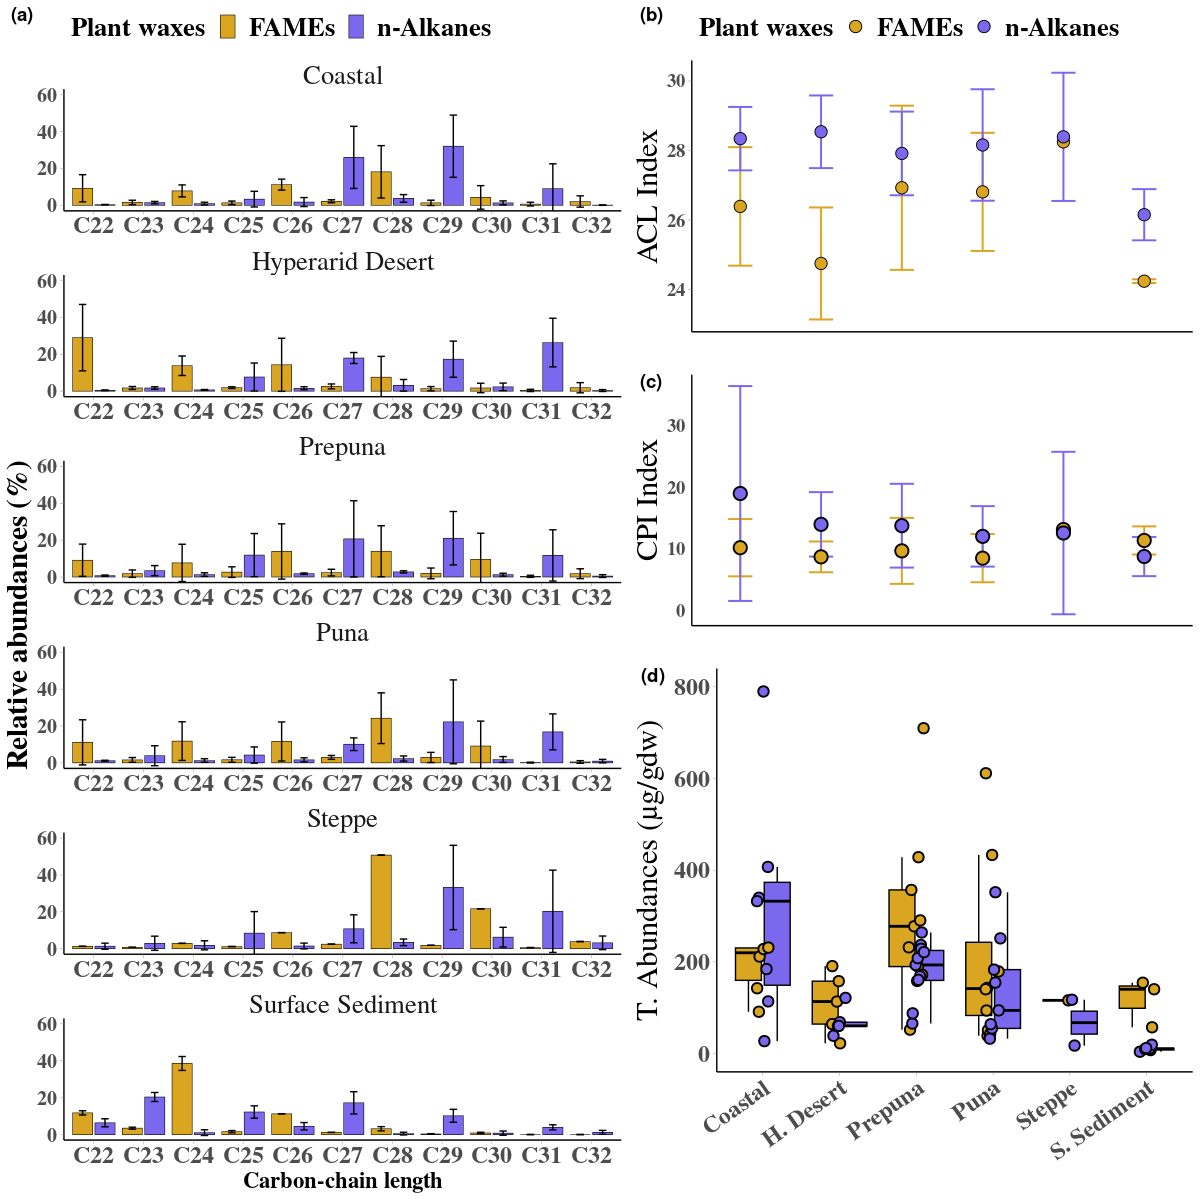
\includegraphics{Fig_2.png}

}

\caption{\label{fig-2}Abundance and distribution of leaf waxes
(\emph{n}-alkanoic acids and \emph{n}-alkanes) along an environmental
gradient in the Atacama Desert (Coast, Hyperarid Desert, pre-Puna, Puna,
Steppe and superficial lacustrine sediments of two high Andean steppe
lakes). (a) average chain length (ACL), (b) carbon preference index
(CPI), (c) Total Abundances and (d) percentage distribution of
long-chain of leaf waxes from twelve species of Atacama Desert.}

\end{figure}

\hypertarget{n-alkanes-and-plant-macrofossils-from-rodent-middens-in-the-atacama-desert-over-the-last-17000-years}{%
\subsection{\texorpdfstring{\emph{n}-Alkanes and plant macrofossils from
rodent middens in the Atacama Desert over the last 17,000
years}{n-Alkanes and plant macrofossils from rodent middens in the Atacama Desert over the last 17,000 years}}\label{n-alkanes-and-plant-macrofossils-from-rodent-middens-in-the-atacama-desert-over-the-last-17000-years}}

A total of sixteen different plant taxa were identified covering twelve
families; fifteen genera and five species of plant macrofossils (Table
1). Radiocarbon ages from 28 rodent middens reveal a temporal coverage
for the last 17 ka cal BP (Table 2). Fecal-pellets indicate that the
middens were made mainly by the ashy chinchilla rat (\emph{Abrocoma
cinerea}) and by leaf-eared mice (\emph{Phyllotis} spp.). In the modern
midden 208-B (150 ± 90 cal yr BP at 3592 m a.s.l., south slope; Table 2)
we find macro-remains of \emph{Haplopappus} sp., \emph{Junellia
bryoides}, \emph{Gilia} sp., \emph{Cistanthe} sp., \emph{Phacelia
cumingii}, \emph{Phacelia pinnatifida}, \emph{Cryptantha} sp. and
\emph{Ephedra americana} ---a composition similar to the species
collected in the field (\emph{Haplopappus} sp., \emph{Junellia
bryoides}, \emph{Gilia} sp., \emph{Cistanthe} sp., \emph{Phacelia}
\emph{cumingii}, \emph{Phacelia pinnatifida}, \emph{Cryptantha} sp. and
\emph{Ephedra americana} besides \emph{Maihueniopsis} sp.,
\emph{Baccharis tola} and \emph{Pappostipa frígida}). Among taxa
identified at the site, we note that some are quite scarce with slope
exclusivities, such as \emph{Maihueniopsis} sp and \emph{Baccharis tola}
on the north slope and \emph{Pappostipa frígida} on the south slope.

A diagram of the relative abundances of each taxon along with the
chronology obtained with AMS \(^{14}\)C dating (Table 2) is shown in
Figure~\ref{fig-3}. The middens were dominated by the local taxa
\emph{Junellia bryoides}, \emph{Cistanthe} sp., \emph{Ephedra americana}
and \emph{Phacelia cumingii}. At ca. 17 ka cal BP, the record shows the
presence of only two local taxa (\emph{Junellia bryoides} and
\emph{Phacelia pinnatifida}) and one extra-local taxa (\emph{Adesmia}
sp.). Between ca. 15.5 and 10 ka cal BP, the record shows an increase in
local plant richness and extra-local species such as \emph{Stipa
frígida}, \emph{Adesmia} sp, \emph{Malvaceae}, \emph{Chenopodiaceae},
\emph{Baccharis aff tola} and \emph{Brassicaceae aff Atacamanivea}. A
large group of middens between ca. 10 and 3 ka cal BP shows a decrease
in plant richness with an increase in the annual extra-local Malvaceae
family. From 3 to 0.18 ka cal BP, there are increases in the local taxa
richness dominated by \emph{Junellia bryoides} and \emph{Cistante} sp.
with the appearance of \emph{Haplopappus} sp. and \emph{Cryptantha} sp.,
among others.

\begin{figure}

{\centering 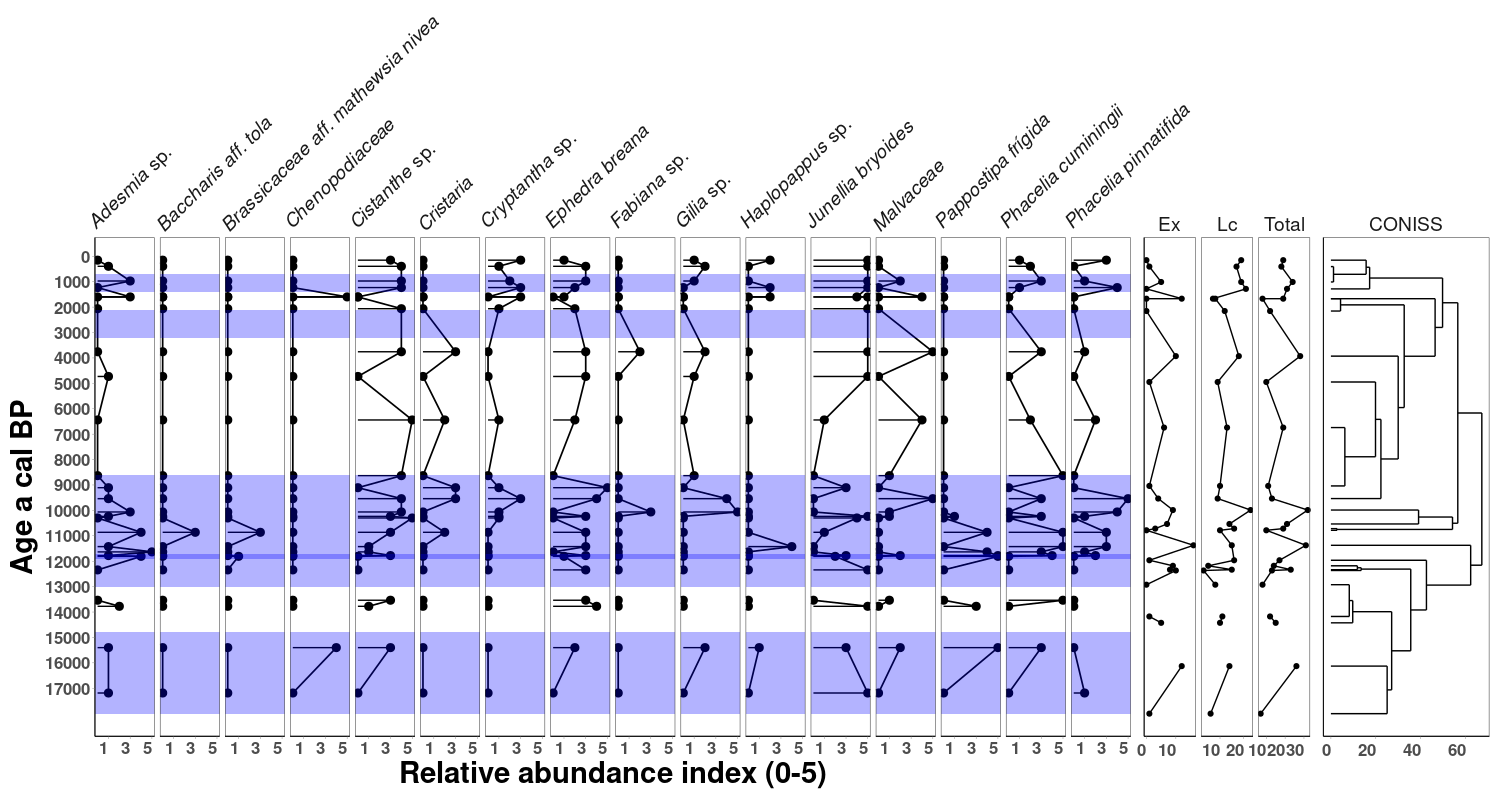
\includegraphics{Fig_3.png}

}

\caption{\label{fig-3}Plant macrofossil diagram from palaeomiddens in
Quebrada Incahuasi. Relative abundance index runs from 0 (absent) to 5
(dominant). Modern analogue groups of local and extralocal taxas have
been defined. Ex: total number of extra-local species, Lc: total number
of local species and ``Total'': represents the total number of species.
A CONISS analysis was performed to see the relationships between the
samples. The purple bands represent of the pluviometric anomalies CAPE I
(ca. 18 to 14.8 ka cal BP), CAPE II (ca. 13.0 to 8.6 and 8.1 to 7.6 ka
cal BP), \textasciitilde2.5 and MCA (ca. 1.2 and 0.8 ka cal BP)
described in the Atacama Desert. Note the different magnitudes of the
abundances.}

\end{figure}

The rodent middens contain high wax values spread with a total mean
\emph{n}-alkanes abundance of 335.4 \(\pm\) 239 \(\mu\)g/gdw (n=24,
\(CPI_{median}\) = 18.46 \(\pm\) 5.44; \(ACL_{median}\) = 29.12 \(\pm\)
0.4, Table 1S and Figure~\ref{fig-4}). The chain-length distribution in
middens was between \emph{n}-\(C_{21}\) and \emph{n}-\(C_{35}\) with a
higher abundance of \emph{n}-\(C_{27}\) to \emph{n}-\(C_{31}\) chain and
predominance of carbon chain length \emph{n}-\(C_{29}\). Fecal-pellet
\(\delta\)\(^{13}\)C values show a range from -21.3 to -25.4
\(\text{\textperthousand}\) with a median of -23
\(\text{\textperthousand}\). The palaeomidden dated to ca. 17 ka cal BP
showed a lower abundance in all chain-length distributions. One of the
main features of the middens dated to ca. 15.2 ka cal BP and between 14
and 12 ka cal BP was the high \emph{n}-alkanes abundances of longer
chains (\emph{n}-\(C_{25}\) to \emph{n}-\(C_{35}\)) compared to the
chain-length abundance between ca. 11 and 5 ka cal BP. The abundances of
\emph{n}-alkanes for the youngest samples dated between 5 and 0.18 ka
cal BP shows an increase in all chain-length distribution, where the
midden with higher \emph{n}-alkanes abundance was at \textasciitilde{} 4
ka cal BP (Figure~\ref{fig-3}). Remarkably, the midden dated at 11.7 ka
cal BP has the highest concentration of \emph{n}-alkanes in the record
(\textasciitilde1,000 \(\mu\)g/gdw), where the carbon length chain
\emph{n}-\(C_{29}\) dominates. Two grass samples, dated between 970
(QIN237-B) and 11,780 (QIN 214b) a cal BP, extracted from the
palaeomiddens matrix showed high \emph{n}-alkane values.

\begin{figure}

{\centering 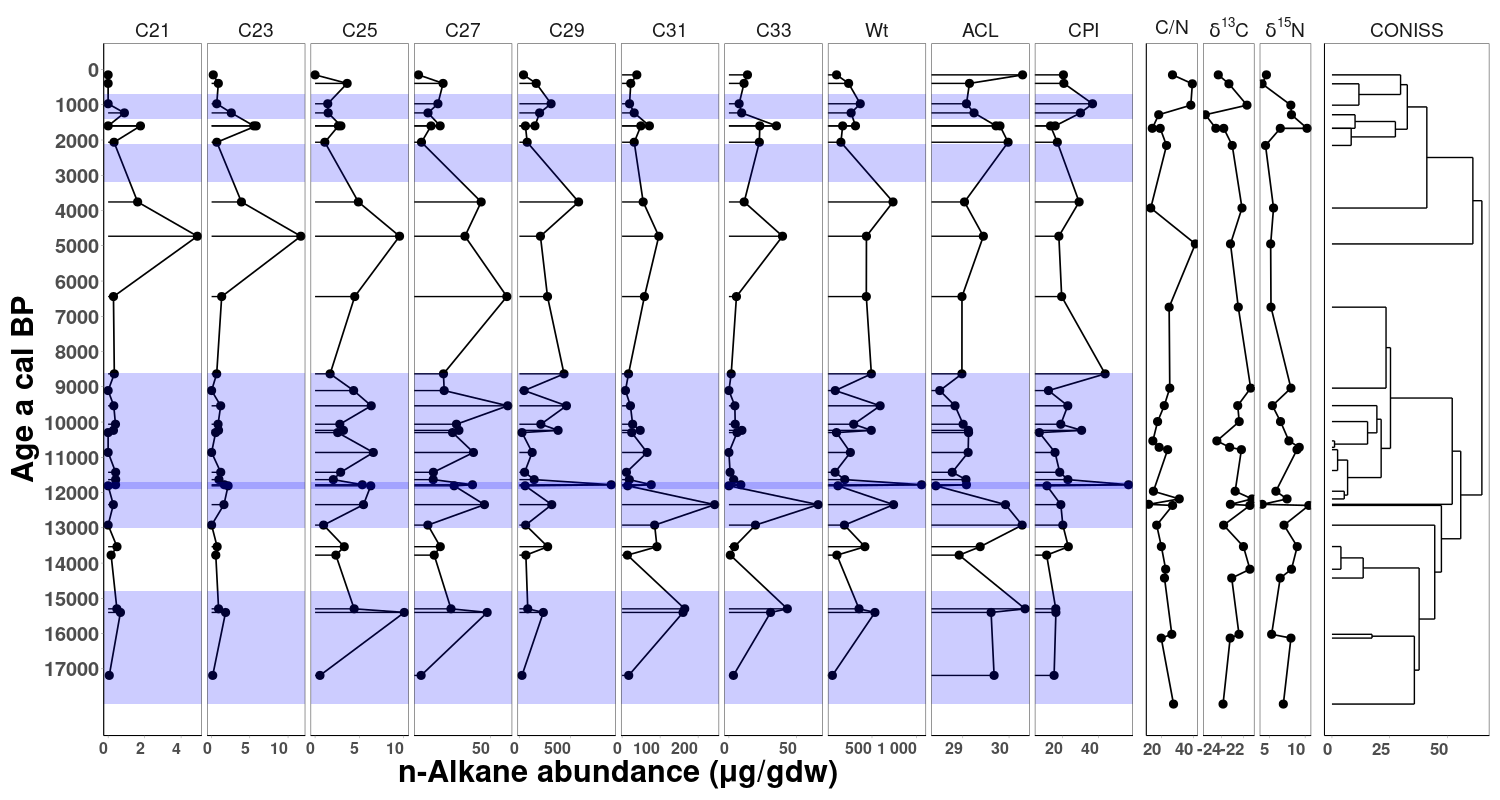
\includegraphics{Fig_4.png}

}

\caption{\label{fig-4}Abundance of \emph{n}-alkanes (\(\mu\)g/gdw) and
\(\delta\)\(^{13}\)C, \(\delta\)\(^{15}\)N and C/N ratio values from
fecal-pellet obtained of the palaeomiddens from Quebrada Incahuasi. A
constrained cluster analysis by the method of incremental sum of squares
(CONISS) was performed to see the relationships between the samples. The
purple bands represent of the pluviometric anomalies CAPE I (ca. 18 to
14.8 ka cal BP), CAPE II (ca. 13.0 to 8.6 and 8.1 to 7.6 ka cal BP),
\textasciitilde2.5 and MCA (ca. 1.2 and 0.8 ka cal BP) described in the
Atacama Desert. Note the different magnitudes of the abundances.}

\end{figure}

\hypertarget{discussion}{%
\section{Discussion}\label{discussion}}

\hypertarget{distribution-of-leaf-wax-n-alkanes-and-n-alkanoic-acids-along-an-altitudinal-transect-504200-m-a.s.l-in-the-atacama-desert}{%
\subsection{\texorpdfstring{Distribution of leaf wax \emph{n}-alkanes
and \emph{n}-alkanoic acids along an altitudinal transect (50--4200 m
a.s.l) in the Atacama
Desert}{Distribution of leaf wax n-alkanes and n-alkanoic acids along an altitudinal transect (50--4200 m a.s.l) in the Atacama Desert}}\label{distribution-of-leaf-wax-n-alkanes-and-n-alkanoic-acids-along-an-altitudinal-transect-504200-m-a.s.l-in-the-atacama-desert}}

The leaf wax \emph{n}-alkanes and \emph{n}-alkanoic acids along the
vegetational transect in the Atacama desert show a species-specific and
heterogeneous distribution in the chain lengths (Figure~\ref{fig-1} and
Figure~\ref{fig-2}). Leaf waxes from Steppe and Puna species have a
clear predominance of \emph{n}-\(C_{29}\)/\emph{n}-\(C_{28}\) chain
lengths in \emph{n}-alkanes and \emph{n}-alkanoic acids, respectively.
On the other hand, the pre-Puna showed a higher abundance on
\emph{n}-\(C_{27}\)/\emph{n}-\(C_{26}\) and
\emph{n}-\(C_{29}\)/\emph{n}-\(C_{28}\) chain lengths. At the coast ---
where advected fog plays an important role as a moisture source --- we
found equal abundance of \emph{n}-\(C_{29}\) and \emph{n}-\(C_{27}\),
while the plants from the Hyperarid Desert showed two different and
antagonistic wax distributions where predominate \emph{n}-alkane
\emph{n}-\(C_{31}\) and a higher \emph{n}-alkanoic acids abundances of
medium chain lengths (Figure~\ref{fig-2}).
\citet{morchenFingerprintPlantLife2021}, found for different plant
species of the Atacama Desert that the \emph{n}-alkane abundances showed
a predominance of chain lengths \emph{n}-\(C_{27}\) and
\emph{n}-\(C_{31}\). These authors related the higher \emph{n}-alkanes
production to the influence of the sources of moisture coming either
from coastal fog or summer precipitation in the Andes.
\citet{contrerasLeafWaxComposition2022} provided a detailed assessment
of \emph{Tillandsia landbeckii} leaf waxes (a CAM species highly
specialized to living only off fog), describing a homogeneous
\emph{n}-alkanes distribution that ranged from \emph{n}-\(C_{23}\) and
\emph{n}-\(C_{31}\) where the leaf wax distribution (ACL and CPI index)
showed a higher inverse correlation with moisture availability. On the
northwestern slope of the south-central Andes of Argentina, soil
\emph{n}-alkanes showed a higher abundance and unimodal distribution
along an altitudinal transect of the chain lengths \emph{n}-\(C_{27}\),
\emph{n}-\(C_{33}\) and \emph{n}-\(C_{29}\)
\citep{nieto-morenoElevationdependentChangesNalkane2016}. While the
tropical forest from Kosñipata valley in Perú,
\citep{feakinsProductionLeafWax2016} showed a predominance of
\emph{n}-\(C_{29}\) and \emph{n}-\(C_{31}\) chains followed by
\emph{n}-\(C_{27}\) and a poor relationship between temperature and leaf
wax distribution. \citet{wuTropicalSoilProfiles2019}, in another
elevation gradient between the Amazon floodplain and the eastern flank
of the Andes in Peru, found a dominance of chain lengths
\emph{n}-\(C_{29}\) and \emph{n}-\(C_{31}\) with a higher
\emph{n}-\(C_{31}\)/\emph{n}-\(C_{29}\) ratio at lower elevation sites.
And \citet{teunissenvanmanenLeafSoilNalkane2020} observed this same
relationship in leaves and soil in Ecuador. All these studies above show
that the proportions in the chain lengths of \emph{n}-alkanes are highly
variable at ecosystem-dependent scale.

Biotic and abiotic stresses can induce metabolic and biosynthesis
responses in cuticular waxes
\citep{shepherdEffectsStressPlant2006, lewandowskaWaxBiosynthesisResponse2020}.
In the Atacama Desert, one of the harshest terrestrial environment
conditions on earth, \emph{n}-alkanes and \emph{n}-alkanoic acids from
leaf-wax show a strong relationship to vegetation belts
(Figure~\ref{fig-1}). We observed a higher total abundance of individual
chains of \emph{n}-alkanes and \emph{n}-alkanoic acids in zones where
the plants have more moisture available coming from the coast and
seasonal summer rains \citep{arroyoEffectsAridityPlant1988}. Atacama
vegetation is adapted to prolonged drought conditions, mechanical
stress, low nutrient availability, and high levels of radiation,
salinity, and metals along the altitude gradient
\citep{diazNitrogenCyclingExtreme2016, rondanelliAtacamaSurfaceSolar2015, eshelPlantEcologicalGenomics2021}.
Several studies show significant correlations between \emph{n}-alkane
distributions with temperature and precipitation
\citep{hoffmannAbundanceDistributionLeaf2013, tippleEnvironmentalControlEastern2013, feakinsProductionLeafWax2016, wangTemperatureEffectAbundance2018},
while others show a weak or null relationship with climatic variables
\citep{carrLeafWaxNalkane2014, howardModellingLeafWax2018}.
\citet{morchenFingerprintPlantLife2021} and
\citet{contrerasLeafWaxComposition2022}, argue that \emph{n}-alkanes
from fog-fed plants in the Atacama that receive coastal moisture show a
dominance of \emph{n}-\(C_{31}\), \emph{n}-\(C_{29}\),
\emph{n}-\(C_{33}\) and \emph{n}-\(C_{27}\) chain lengths, whereas
plants affected by summer rainfall show a greater abundance of
\emph{n}-\(C_{31}\) and \emph{n}-\(C_{29}\) chain lengths. The
\emph{n}-alkane distributions along the Atacama Desert suggests a strong
relationship with the available moisture conditions in the vegetation
belts, which should be evaluated before using the leaf waxes as an
indicator of paleoenvironmental change.

\hypertarget{sources-n-alkane-leaf-wax-in-a-17000-yr-long-rodent-midden-record-from-atacama-desert}{%
\subsection{\texorpdfstring{Sources \emph{n}-alkane leaf wax in a 17,000
yr long rodent midden record from Atacama
Desert}{Sources n-alkane leaf wax in a 17,000 yr long rodent midden record from Atacama Desert}}\label{sources-n-alkane-leaf-wax-in-a-17000-yr-long-rodent-midden-record-from-atacama-desert}}

The analysis of \emph{n}-alkanes in rodent coprolites from middens show
a marked distribution range of chain length between \emph{n}-\(C_{21}\)
and \emph{n}-\(C_{35}\) with a greater abundance of \emph{n}-\(C_{29}\)
followed by \emph{n}-\(C_{31}\) (Figure~\ref{fig-4}). These wax
distributions are similar to those found in plants that dominate the
Steppe and Puna, where species such as \emph{Pappostipa frigida},
\emph{Haplopappus rigidus} and \emph{Junellia seriphioides} have a
greater abundance of \emph{n}-\(C_{27}\), \emph{n}-\(C_{29}\) and
\emph{n}-\(C_{31}\). In the Steppe, where \emph{Pappostipa frigida}
dominates the landscape, the fingerprint of chain length is the
\emph{n}-\(C_{29}\). When we compare the \emph{n}-alkanes from grasses
inside two rodent middens matrix with the \emph{n}-alkanes obtained from
their fecal-pellet (QIN237-B and QIN214-B; ca. 970 and 11,780 a cal BP,
respectively), we note a similar pattern between their distributions
(Figure 5S), but with concentrations that are one to two orders of
magnitude lower ---50/16 \(\mu\)g/gdw in grasses compared to 368/1054
\(\mu\)g/gdw in fecal-pellet (Figure~\ref{fig-4}).
\citet{latorreVegetationInvasionsAbsolute2002}, studied the relationship
between vegetation and dietary behavior by analyzing cuticles in feces
from 41 rodent middens during the last 45 ka cal BP of the pre-Puna of
the Atacama Desert. This comparative study between plant macrofossil,
abundance of grasses and leaf wax analysis showed that the diets of
different rodent species are closely related to the surrounding
vegetation, however, we cannot rule out that the dietary preferences and
collecting behaviors can introduce bias into midden records
\citep{borrelliDietaryModificationsPackrats2016}. Our fecal-pellet
isotopic analysis shows \(\delta\)\(^{13}\)C values close to -23
\(\text{\textperthousand}\) that are indicative of an almost pure
\(C_{3}\) diet \citep{latorreVegetationInvasionsAbsolute2002}. This is
consistent with our RDA analysis between plant macrofossil and
\emph{n}-alkane abundance, which separates the abundance of
\emph{n}-\(C_{29}\) and plant extralocal from \emph{n}-\(C_{31}\) and
local taxa of the pre-Puna (Figure 6S). Based on our observations, we
predict that a higher abundance of plant species in the landscape will
lead to increased variation in chain length distributions in
palaeomiddens. In addition, we expect to see a pronounced dominance of
\emph{n}-\(C_{29}\) during periods of increased grass abundance. This
observation can be explained by the presence of species-specific
chemotaxonomic biomarkers and the generalist dietary behaviour of
rodents
\citep{latorreVegetationInvasionsAbsolute2002, borrelliDietaryModificationsPackrats2016}.

\hypertarget{leaf-wax-n-alkane-in-rodent-midden-record-as-proxy-of-palaeoenvironmental-changes}{%
\subsection{\texorpdfstring{Leaf wax \emph{n}-alkane in rodent midden
record as proxy of palaeoenvironmental
changes}{Leaf wax n-alkane in rodent midden record as proxy of palaeoenvironmental changes}}\label{leaf-wax-n-alkane-in-rodent-midden-record-as-proxy-of-palaeoenvironmental-changes}}

Palaeomidden records from the central Atacama (15\(^\circ\) to
27\(^\circ\)S), contain many extra-local species indicative of past
pluvials in the south-central Andes during the Quaternary
\citep{betancourt22000YearRecord2000, rechLateQuaternaryPaleohydrology2002, latorreLateQuaternaryVegetation2006, diazMultiscaleClimateChange2019}.
At least six pluviometric anomalies have been linked with vegetation
changes in the Atacama; CAPE I (ca. 18 to 14.8 ka cal BP), CAPE II (ca.
13.0 to 8.6 and 8.1 to 7.6 ka cal BP) and four relatively short-period
pluvials during \textasciitilde{} 4 to 3.4, \textasciitilde2.5, MCA (ca.
1.2 and 0.8 ka cal BP) and LIA (ca. 0.5 and 0.1 ka cal BP). Low latitude
insolation changes and/or strengthening/weakening of the South American
Monsoon System and precipitation from the maritime weather system
---forced by ocean-atmosphere dynamics of the Pacific and/or Atlantic---
are the most common climatic teleconnections proposed to explain these
precipitation anomalies
\citep{betancourt22000YearRecord2000, rechLateQuaternaryPaleohydrology2002, gayoLateQuaternaryHydrological2012, gonzalez-pinillaHighLowlatitudeForcings2021}

Can the \emph{n}-alkanes obtained from palaeomidden records reflect
niche shifts in the Atacama plant communities during the past? The leaf
wax \emph{n}-alkane chain-length distributions of the plants studied
show a clear species-specific molecular signature associated with the
different vegetational belts (Figure 2S). High Andean Steppes from
Atacama are represented mainly by \emph{n}-\(C_{29}\) and
\emph{n}-\(C_{31}\) \emph{n}-alkanes. At the same time, environments in
lowlands (pre-Puna and Puna) are characterized by a greater diversity of
chain lengths between \emph{n}-\(C_{22}\) to \emph{n}-\(C_{33}\) due to
the different species that live there. These molecular relationships
could be used to detect wax input due to extra-local species in ancient
Atacama ecosystems. In that regard, rodent palaeomiddens can be an
excellent tool to understand the relationships between wax production
and plant species that lived at a given time. Plant macrofossils
analysis from modern middens dated around 150 cal a BP (3592 m asl,
Figure~\ref{fig-3}) from pre-Puna showed a composition similar to the
species collected in the field (\emph{Haplopappus} sp, \emph{Junellia
bryoides}, \emph{Gilia} sp, \emph{Cistanthe} sp, \emph{Phacelia
cumingii}, \emph{Phacelia pinnatifida}, \emph{Cryptantha} sp. and
\emph{Ephedra americana}). In the same manner, as observed in the Puna
and pre-Puna, the \emph{n}-alkanes chain lengths obtained from
fecal-pellets in these modern middens are dominated by
\emph{n}-\(C_{25}\), \emph{n}-\(C_{27}\) and \emph{n}-\(C_{33}\) whereas
\emph{n}-\(C_{29}\) and \emph{n}-\(C_{31}\) are co-dominants.
Furthermore, when we analyze the \emph{n}-alkane distributions across
all palaeomiddens over the last 17 ka cal BP, the data show a high
variability in n-alkane chain lengths (Figure~\ref{fig-4}). We propose
that these heterogeneous \emph{n}-alkane distributions represent a
response to changes in the climate and species composition of the
pre-Puna where the palaeomiddens are generated. That idea is supported
by the redundancy analysis (RDA) where the extra-local species are
grouped with \emph{n}-\(C_{25}\), \emph{n}-\(C_{27}\) and
\emph{n}-\(C_{29}\) \emph{n}-alkanes (Figure 6S) and by the link between
the \emph{n}-alkane distributions of grasses and fecal-pellets found in
the middens QIN237-B and QIN214-B (Figure 5S). This suggests that the
Atacama Desert plants have a sufficiently high molecular plasticity to
overrun ecosystems different from the current, as shown by some recent
studies in these extreme habitats
\citep{diazMultiscaleClimateChange2019, eshelPlantEcologicalGenomics2021, dussarratPredictiveMetabolomicsMultiple2022}.
To test this assumption, we compare our \emph{n}-alkanes palaeomidden
series with different climate change records associated with flood
variations in the Atacama Desert (Figure~\ref{fig-5}).

\newpage{}

\begin{figure}

{\centering 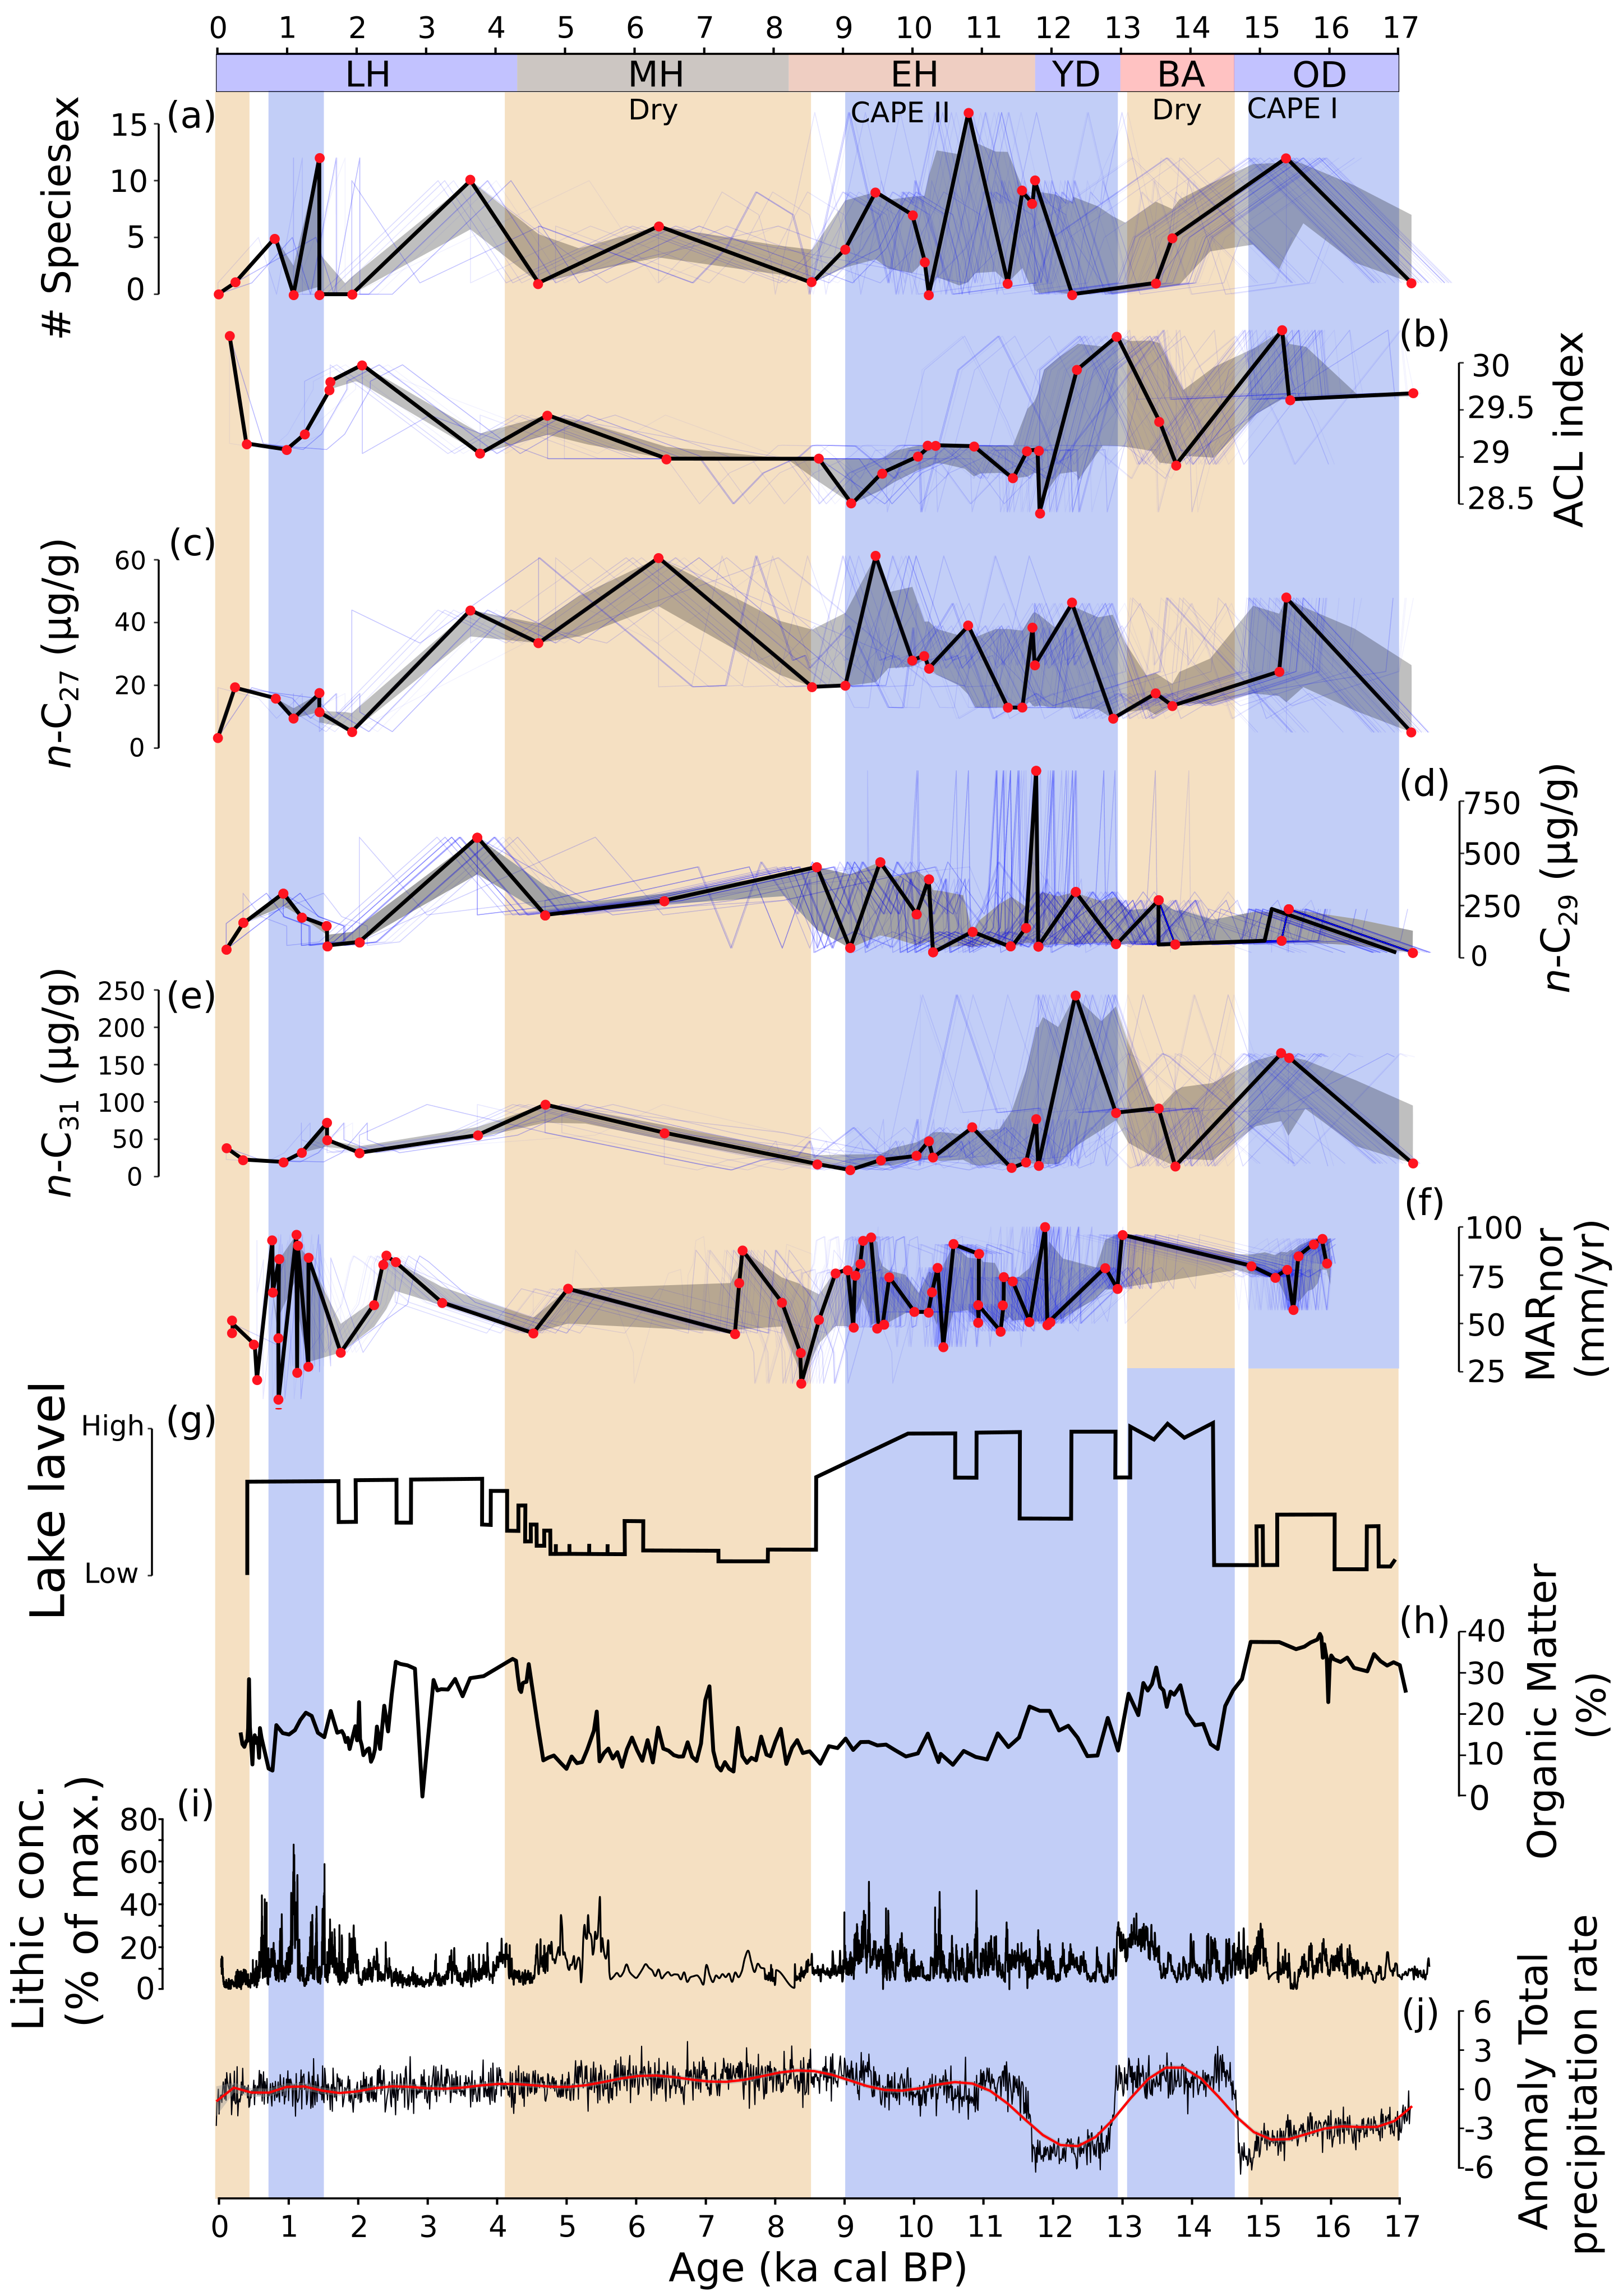
\includegraphics{Fig_5.png}

}

\caption{\label{fig-5}Comparison of selected \emph{n}-alkane abundances
and macrofossil obtained from palaeomidden records with representative
local, regional and global palaeoclimate records. (a) total number of
extra-local species of macrofossil from palaeomiddens in Quebrada
Incahuasi. (b) average chain length (ACL) of \emph{n}-alkanes. (c-e)
\emph{n}-\(C_{27}\), \emph{n}-\(C_{29}\) and \emph{n}-\(C_{31}\)
\emph{n}-alkane abundances (\(\mu\)g/gdw). (f) MAR anomalies in the
central Atacama Desert (González-Pinilla et al., 2021). (g) Miscanti
ancient lake level (Valero-Garcés et al., 1996; Grosjean et al., 2001,
23º44'S, 67º46'W, 4140 m asl). (h) Amount of organic matter from Junín
lake (Rodbell et al.,, 2022, 4080 m asl ).(i) Late Pleistocene-Holocene
El Niño-like ENSO-sensitive marine records, from Peruvian shelf (Rein et
al., 2005). (j) Transient simulation of precipitation (TraCE 21k-II, (He
and Clark, 2022) over the central Atacama (24°S). From (a) to (f), the
age-uncertainty median ensemble (estimated with the Banded Age Model in
GeochronR package) is shown in black, with the 50\(\%\) and 95\(\%\)
highest-density probability ranges shown in dark and light gray,
respectively. (see Comboul et al., 2014; McKay et al., 2021 for more
detail). OD: Oldest Dryas, BA: Bølling-Allerød, YD: Younger Dryas
Stadial.}

\end{figure}

\newpage{}

During the CAPE I, palaeomidden records show an increase of extra-local
species, together with \emph{n}-\(C_{25}\), \emph{n}-\(C_{27}\),
\emph{n}-\(C_{29}\) and \emph{n}-\(C_{33}\) \emph{n}-alkanes
(Figure~\ref{fig-4} and Figure~\ref{fig-5} a-d). According to the
current distribution of chain lengths in the Atacama Desert, this
increase could represent greater biodiversity of plants from different
vegetation belts. \citet{gonzalez-pinillaHighLowlatitudeForcings2021},
reconstructed positive mean annual rainfall (MAR) anomalies in the
Atacama Desert at 15.9 to 14.8 ka cal BP (MAR = 142 \(\pm\) 10), 13.0 to
8.6 ka B.P (MAR = 130 \(\pm\) 18) and more variable precipitation during
the Late Holocene (Figure~\ref{fig-5} f). They associated the MAR
anomalies from CAPE I to the Heinrich Event 1 (HE-1) and La Niña-like
conditions inferred from El Niño flood activity record in Perú
\citep{reinNinoVariabilityPeru2005} that drove an intensification and
southward shift of the South American Summer Monsoon (SASM). These
moisture changes are coeval with those observed in the \emph{n}-alkanes
of the midden series (Figure~\ref{fig-5} f). In contrast, in the western
Central Andes lake records (Figure~\ref{fig-5} h-g), there are low lake
levels at lakes of Miscanti, Chungará and Junín during this phase, which
have been associated with the weakening of the SASM and the hydrological
balance of the upper Amazon basin and the Altiplano
\citep{valero-garcesLimnogeologyLagunaMiscanti1996, moreno14kyrRecordTropical2007a, rodbell700000Years2022}.
During the CAPE II, the \emph{n}-alkanes show an initial increase in
\emph{n}-\(C_{31}\) chain length followed by an abrupt increase in
\emph{n}-\(C_{29}\) during the end of the YD (at ca. 10.8 ka cal BP)
followed by fluctuations of the \emph{n}-\(C_{27}\) \emph{n}-alkane
(Figure~\ref{fig-5}). Between the CAPE I and CAPE II phases (ca. 14.8
and 13.1 ka BP), the decrease of \emph{n}-alkanes are indicative of dry
conditions that coincide with the Bölling/Allerød (BA) warming period
and the Meltwater Pulse 1A (MWP-1A) occurred around 14.6 ka
\citep{liuTransientSimulationLast2009, obaseAbruptBollingAllerodWarming2019, heFreshwaterForcingAtlantic2022}.
These data support the assumption of a very dry period by
\citet{gonzalez-pinillaHighLowlatitudeForcings2021} between 14.8 and
13.1 ka B.P. However, high lake levels in the western central Andes
(Figure~\ref{fig-5} g-f) during this period suggest a seesaw response of
the SASM, possibly related to meridional shifts of the Intertropical
Convergence Zone (ITCZ) forcing by Atlantic Meridional Overturning
Circulation (AMOC) and North Atlantic SST variability during the last
deglaciation \citep[see Figure~\ref{fig-5}
j]{fornace60000yearRecord2014a}. A weaker AMOC reduces northward energy
transport, leading to cooler North Atlantic SSTs. This can cause the
ITCZ to shift southward, as it tends to follow the region of maximum
SSTs and associated convection. A southward shift of the ITCZ in turn
affects the strength and position of the South Atlantic Subtropical
Anticyclone and the position of the trade winds in the tropical
Atlantic, leading to a redistribution of rainfall within the tropics and
subtropics, with less rainfall further north and more rainfall further
south
\citep{schneiderMigrationsDynamicsIntertropical2014a, houstonRoleNonstationaryAndean2022}.
However, the direct impact of the AMOC on the Atacama Desert is likely
to be limited. This apparent disagreement could be explained by
different sources of oceanic and continental moisture along the Andean
Dry Diagonal, where ENSO-like conditions could play a predominant role
\citep[see][]{houstonRoleNonstationaryAndean2022}. Stable deuterium and
carbon isotope analysis of individual long-chain \emph{n}-alkanes from
palaeomiddens could give us clues about the mechanisms at work in the
Atacama Desert. In the Middle Holocene, the paloemidden record shows a
greater abundance of \emph{n}-\(C_{29}\) and \emph{n}-\(C_{27}\) chain
lengths typical of grasses, while during the Late Holocene the
differences in abundances among the \emph{n}-alkanes decrease. Several
authors have described arid conditions in the Atacama Desert during the
Middle Holocene
\citep{grosjeanLateglacialEarlyMiddle1994, valero-garcesLimnogeologyLagunaMiscanti1996, betancourt22000YearRecord2000, nunezHumanOccupationsClimate2002a},
the timing and lapse of this aridity condition are still under
discussion
\citep{grosjeanMidHoloceneClimateSouthCentral2001, latorreVegetationInvasionsAbsolute2002, rechLateQuaternaryPaleohydrology2002},
where La Niña-like conditions and spatially complex SASM system
precipitation are the main characteristics
\citep{reinNinoVariabilityPeru2005, wongVariationsSouthAtlantic2021}.
Finally, during the Late Holocene the \emph{n}-alkanes chain lengths are
co-dominant and represent the present-day plant communities, where
climatic variability could only partly explain present-day chain length
distributions if we consider other factors such as species introduction
by human activity.

\hypertarget{conclusions}{%
\section{Conclusions}\label{conclusions}}

This work demonstrates how the abundance of leaf waxes and records of
climate change obtained from palaeomiddens are related to vegetation
change in the Atacama. The \emph{n}-alkanes and \emph{n}-alkanoic acids
from current plant leaf waxes show a high variability through the
elevational gradient and a species-specific molecular signature of these
vegetational belts. The Steppe is characterized by high abundances of
\emph{n}-\(C_{29}\) chain length followed by \emph{n}-\(C_{31}\) and
\emph{n}-\(C_{27}\), respectively. Leaf waxes from the Puna and pre-Puna
have a greater abundance and diversity of chain lengths, whereas in the
absolute desert the most abundant \emph{n}-alkanes and \emph{n}-alkanoic
acids are the \emph{n}-\(C_{31}\) and \emph{n}-\(C_{22}\) chains. Along
the coastal Atacama, the \emph{n}-alkanes that predominated are
\emph{n}-\(C_{27}\) and \emph{n}-\(C_{29}\) in contrast with a decrease
of the \emph{n}-alkanoic acids that are dominated by \emph{n}-\(C_{28}\)
and \emph{n}-\(C_{26}\) chains. We observe a decoupling of leaf wax ACL
values between \emph{n}-alkanes and \emph{n}-alkanoic acids in the
absolute desert. Biochemical differences between \emph{n}-alkanes and
\emph{n}-alkanoic acids ACL values could imply different hydric-deficit
tolerance strategies in plants under hyper-extreme environmental
conditions. In general, our study shows that palaeomiddens are an
excellent source of leaf wax abundances in the pre-Puna of the Atacama
and respond to different moisture pulses previously identified in the
region. As described in other research, the palaeomidden record
indicates increased wet conditions during the CAPE phases consistent
with lower summer insolation and increased humidity modulated by ENSO
and SASM. Furthermore, palaeomiddens show a dry period between ca. 13
and 14.8 ka cal BP co-occurring during a strengthened AMOC and abrupt
increase in grasses at 11.7 ka cal BP as indicated by increased
abundance of \emph{n}-\(C_{29}\) chain length. Lower bioproductivity
could be interpreted during the Early and Middle Holocene (from ca. 11.0
to 6.0 ka cal BP), coincident with a decrease in precipitation described
for the Atacama. Multiple interrelations between solar irradiance,
climate, nutrient and vegetational changes could be controlling the
abundance of waxes in time, and other proxies should be used to confirm
this relationship. However, more comprehensive leaf wax analysis of the
dominant vegetation and other midden series are required to better
understand and quantify the link between climatic variability and
\emph{n}-alkyl leaf waxes under extreme arid environmental conditions.
These records create an opportunity to complement other palaeoclimate
proxies with isotopic analysis and genetic information across a wide
spatial range to understand the complex relationships between climate
and desert vegetation where other palaeoclimate records are scarce.

\hypertarget{data-availability}{%
\section{Data Availability}\label{data-availability}}

All raw data and code used in this paper are publicly available for
reuse via Zenodo (doi:10.5281/zenodo.7768860) and Github
(https://github.com/mat1506/atacama.waxes.git)

\hypertarget{acknowledgments}{%
\section{Acknowledgments}\label{acknowledgments}}

We thank Chris Moy, Jean Pierre Francois, Hector Orellana, the
indigenous community of Socaire and CONAF for help with sample analysis
and logistical support in the field.

\hypertarget{financial-support}{%
\section{Financial support}\label{financial-support}}

This research was supported by the ANID-FONDECYT (grants 1190398,
1191568, 11220930, 3180368). Additional support was provided by the
Millennium Science Initiative Program Nucleus AFOREST (NCS2022\_24) and
the Millennium Science Initiative Nucleus UPWELL (NCN19-153) of the
Ministry of Economy, Development and Tourism (Chile) and IEB (through
ANID FB210006).

\hypertarget{credit-authorship-contribution-statemen}{%
\section{CRediT authorship contribution
statemen}\label{credit-authorship-contribution-statemen}}

The authors declare that they have no conflict of interest

\newpage{}

\hypertarget{tables}{%
\section{Tables}\label{tables}}

\textbf{Table 1: Macrofossils identified, including their family, type
and phytogeographic affinity.}

\textbf{Table 2: Site location, radiocarbon dates, calendar year BP
(95.4}\(\%\) probability ranges; curve Shcal20, Oxcal 4.4) and former
agent for 28 rodent middens analyzed (see Fig. 1 for midden localities).
\emph{SD}: standard deviation, *:Unidentified

\newpage{}


\renewcommand\refname{References}
  \bibliography{bibliography.bib}


\end{document}
